% ============================================================================
% Lecture 06 (B05): Deep Equilibrium Nets --- The Central Idea
% Deep Learning for Solving and Estimating Dynamic Models in Economics and Finance
% Course author: Simon Scheidegger
% ============================================================================

\documentclass[aspectratio=169,11pt]{beamer}

% ---------- Theme and colors ----------
\usecolortheme{dove}
\setbeamertemplate{navigation symbols}{}
\setbeamertemplate{footline}{%
  \hfill\usebeamerfont{page number in head/foot}%
  \usebeamercolor[fg]{normal text}%
  \insertframenumber\,/\,\inserttotalframenumber\kern1em\vskip4pt}
\setbeamerfont{frametitle}{size=\huge}

% ---------- Packages ----------
\usepackage[utf8]{inputenc}
\usepackage[T1]{fontenc}
\usepackage{amsmath,amssymb,amsfonts}
\usepackage{bm}
\usepackage{graphicx}
\usepackage{tikz}
\usetikzlibrary{shapes,arrows.meta,positioning,calc,fit,backgrounds,patterns,decorations.pathreplacing}
\usepackage{pgfplots}
\pgfplotsset{compat=1.18}
\usepackage{booktabs}
\usepackage{hyperref}
\usepackage{multicol}
\usepackage{xcolor}
\usepackage{algorithm}
\usepackage{algorithmic}

% ---------- Custom colors ----------
\definecolor{uzhblue}{rgb}{0,0,0.5}
\definecolor{uzhgreylight}{RGB}{236,238,241}
\definecolor{uzhgreydark}{RGB}{81,86,94}
\definecolor{harvardcrimson}{RGB}{153,0,0}
\definecolor{unil@blue}{RGB}{0,140,204}
\definecolor{unil@black}{RGB}{35,31,32}
\definecolor{darkgreen}{RGB}{0,100,0}
\definecolor{darkred}{RGB}{139,0,0}
\definecolor{softblue}{RGB}{70,130,180}
\definecolor{softorange}{RGB}{230,159,0}
\definecolor{softgreen}{RGB}{0,158,115}

% ---------- Set beamer colors ----------
\setbeamercolor{frametitle}{bg=uzhgreylight, fg=uzhblue}
\setbeamercolor{title}{fg=uzhblue}
\setbeamercolor{structure}{fg=uzhblue}
\setbeamercolor{block title}{bg=unil@blue, fg=white}
\setbeamercolor{block body}{bg=uzhgreylight}
\setbeamercolor{block title alerted}{bg=darkred,fg=white}
\setbeamercolor{block body alerted}{bg=red!5}
\setbeamercolor{block title example}{bg=darkgreen,fg=white}
\setbeamercolor{block body example}{bg=green!5}
\setbeamercolor{item}{fg=unil@black}
\setbeamercolor{normal text}{fg=unil@black}

% ---------- Emphasis and hyperlinks ----------
\newcommand{\emphc}[1]{\textcolor{harvardcrimson}{#1}}
\hypersetup{colorlinks,linkcolor=harvardcrimson,urlcolor=harvardcrimson}

% ---------- Math commands ----------
\newcommand{\x}{\bm{x}}
\newcommand{\w}{\bm{w}}
\newcommand{\bb}{\bm{b}}
\newcommand{\z}{\bm{z}}
\newcommand{\W}{\bm{W}}
\newcommand{\X}{\bm{X}}
\renewcommand{\a}{\bm{a}}
\newcommand{\R}{\mathbb{R}}
\newcommand{\E}[1]{\mathbb{E}\!\left[#1\right]}
\DeclareMathOperator*{\argmin}{arg\,min}
\DeclareMathOperator*{\argmax}{arg\,max}

% ---------- Title ----------
\title[Lecture 07 (B06)]{Lecture 07 (B06): Brock--Mirman with DEQNs --- Deterministic Case}
\subtitle{Neural network architecture, supervised vs unsupervised, deterministic Brock--Mirman}
\author{Simon Scheidegger}
\institute{HEC, University of Lausanne}
\date{}
\begin{document}

% Custom command used in some "Finger Exercise" frame titles.
\providecommand{\exercisepause}{%
  \tikz[baseline=(X.base)]{\node[fill=darkgreen!80!black, text=white,
  rounded corners=2pt, inner sep=3pt, font=\scriptsize\bfseries](X){PAUSE};}}

{\setbeamercolor{background canvas}{bg=uzhgreylight}
\begin{frame}
\titlepage
\end{frame}
}

% --- About-this-lecture orientation ---
\begin{frame}{About this lecture}
\small
\begin{block}{What this lecture covers}
\begin{itemize}\itemsep2pt
  \item Neural-network architecture for DEQNs: layer structure, activations, supervised vs unsupervised framing
  \item The Brock-Mirman deterministic growth model: setup, Euler equation, closed-form policy
  \item End-to-end DEQN training pass on a model whose true solution is known analytically
\end{itemize}
\end{block}
\begin{block}{Builds on}
\begin{itemize}\itemsep2pt
  \item Lecture 06 (DEQN central idea)
  \item Lectures 03-05 (training mechanics, loss design)
\end{itemize}
\end{block}
\begin{block}{Leads to}
\begin{itemize}\itemsep2pt
  \item Lecture 08 (adding stochastic shocks; Gauss-Hermite quadrature)
  \item Lecture 09 (constraints and loss kernels)
\end{itemize}
\end{block}
\end{frame}

\begin{frame}{What is a Deep Neural Network?}
A deep neural network (DNN) $\mathcal{N}_\rho : \R^{d_{\text{in}}} \to \R^{d_{\text{out}}}$ is a \emphc{parametric function approximator}.

\vspace{0.5em}
\textbf{Universal approximation} (Cybenko 1989, Hornik et al.\ 1989):
\[
\forall f \in C(\mathcal{K},\R),\ \forall\varepsilon > 0,\;\; \exists\, \rho^\star : \quad \sup_{\x\in\mathcal{K}}\bigl\|\mathcal{N}_{\rho^\star}(\x) - f(\x)\bigr\| < \varepsilon
\]
{\scriptsize ($\mathcal{K}\subset\R^{d_{\mathrm{in}}}$ compact; the norm is the supremum over $\mathcal{K}$.)}

\vspace{0.5em}
\textbf{In economics:}
\begin{itemize}
    \item \emphc{Input:} state variables $\x_t \in \R^{d}$ (capital, productivity, wealth distribution, \ldots)
    \item \emphc{Output:} policy variables (consumption, savings, prices, \ldots)
    \item \emphc{Parameters} $\rho$: weights and biases, found by \emphc{training}
\end{itemize}
\end{frame}

% --- Slide 13: DNN Layer Structure ---
\begin{frame}{DNN Layer Structure}
\begin{center}
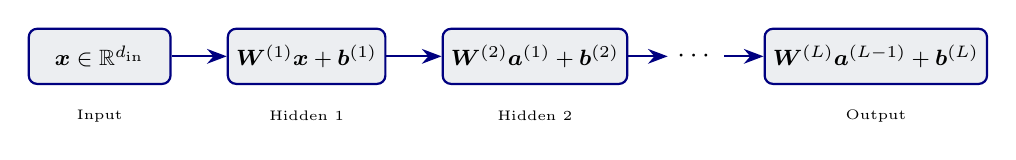
\begin{tikzpicture}[
    mlstep/.style={rectangle, draw=uzhblue, thick, fill=uzhgreylight,
        minimum width=1.8cm, minimum height=0.7cm, font=\footnotesize,
        rounded corners=3pt, inner sep=3pt},
    arr/.style={-{Stealth[length=2.5mm]}, thick, uzhblue}
]
    \node[mlstep] (in) {$\x \in \R^{d_{\text{in}}}$};
    \node[mlstep, right=0.7cm of in] (h1) {$\W^{(1)}\x + \bb^{(1)}$};
    \node[mlstep, right=0.7cm of h1] (h2) {$\W^{(2)}\a^{(1)} + \bb^{(2)}$};
    \node[right=0.5cm of h2, font=\normalsize] (dots) {$\cdots$};
    \node[mlstep, right=0.5cm of dots] (out) {$\W^{(L)}\a^{(L-1)} + \bb^{(L)}$};

    \draw[arr] (in) -- (h1);
    \draw[arr] (h1) -- (h2);
    \draw[arr] (h2) -- (dots);
    \draw[arr] (dots) -- (out);

    \node[below=0.2cm, font=\tiny] at (in.south) {Input};
    \node[below=0.2cm, font=\tiny] at (h1.south) {Hidden 1};
    \node[below=0.2cm, font=\tiny] at (h2.south) {Hidden 2};
    \node[below=0.2cm, font=\tiny] at (out.south) {Output};
\end{tikzpicture}
\end{center}

\vspace{0.4em}
Each layer performs an \emphc{affine transformation}:
\[
\z^{(\ell)} = \W^{(\ell)} \a^{(\ell-1)} + \bb^{(\ell)}, \qquad \ell = 1, \ldots, L
\]
where $\W^{(\ell)} \in \R^{n_\ell \times n_{\ell-1}}$ and $\bb^{(\ell)} \in \R^{n_\ell}$.

\vspace{0.3em}
{\small Without nonlinear activations, the entire network collapses to a single affine map.}
\end{frame}

% --- Slide 14: Activation Functions ---
\begin{frame}{Activation Functions}
\begin{center}
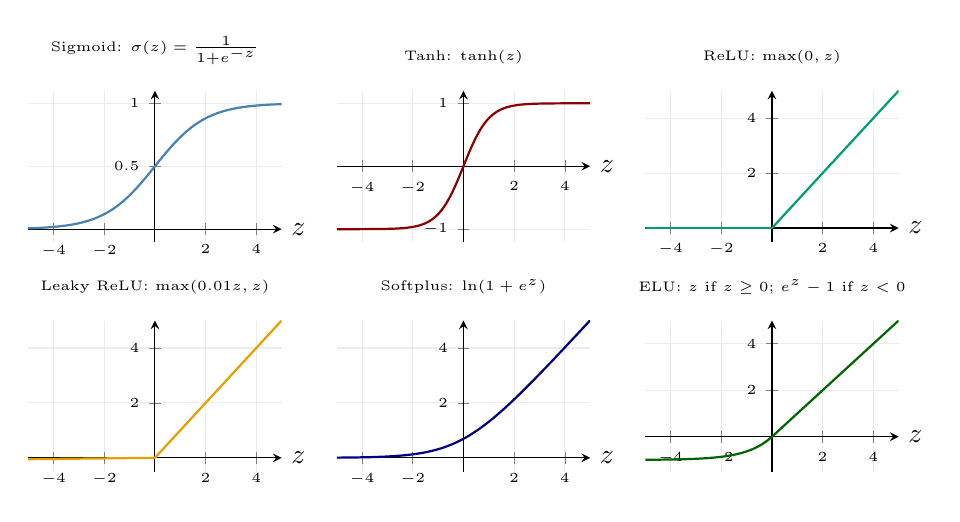
\begin{tikzpicture}
% Row 1: Sigmoid, Tanh, ReLU
\begin{axis}[
    name=plot1,
    width=4.8cm, height=3.5cm,
    title={\tiny Sigmoid: $\sigma(z) = \frac{1}{1+e^{-z}}$},
    title style={font=\tiny},
    xlabel={$z$}, xlabel style={font=\tiny},
    tick label style={font=\tiny},
    xmin=-5, xmax=5, ymin=-0.1, ymax=1.1,
    grid=major, grid style={gray!15},
    axis lines=middle,
    every axis x label/.style={at={(current axis.right of origin)}, anchor=west},
]
    \addplot[thick, softblue, domain=-5:5, samples=100]{1/(1+exp(-x))};
\end{axis}

\begin{axis}[
    at={($(plot1.east)+(0.7cm,0)$)}, anchor=west,
    name=plot2,
    width=4.8cm, height=3.5cm,
    title={\tiny Tanh: $\tanh(z)$},
    title style={font=\tiny},
    xlabel={$z$}, xlabel style={font=\tiny},
    tick label style={font=\tiny},
    xmin=-5, xmax=5, ymin=-1.2, ymax=1.2,
    grid=major, grid style={gray!15},
    axis lines=middle,
    every axis x label/.style={at={(current axis.right of origin)}, anchor=west},
]
    \addplot[thick, darkred, domain=-5:5, samples=100]{tanh(x)};
\end{axis}

\begin{axis}[
    at={($(plot2.east)+(0.7cm,0)$)}, anchor=west,
    name=plot3,
    width=4.8cm, height=3.5cm,
    title={\tiny ReLU: $\max(0,z)$},
    title style={font=\tiny},
    xlabel={$z$}, xlabel style={font=\tiny},
    tick label style={font=\tiny},
    xmin=-5, xmax=5, ymin=-0.5, ymax=5,
    grid=major, grid style={gray!15},
    axis lines=middle,
    every axis x label/.style={at={(current axis.right of origin)}, anchor=west},
]
    \addplot[thick, softgreen, domain=-5:0, samples=2]{0};
    \addplot[thick, softgreen, domain=0:5, samples=2]{x};
\end{axis}

% Row 2: Leaky ReLU, Softplus, ELU
\begin{axis}[
    at={($(plot1.south)-(0,1.0cm)$)}, anchor=north,
    name=plot4,
    width=4.8cm, height=3.5cm,
    title={\tiny Leaky ReLU: $\max(0.01z,z)$},
    title style={font=\tiny},
    xlabel={$z$}, xlabel style={font=\tiny},
    tick label style={font=\tiny},
    xmin=-5, xmax=5, ymin=-0.5, ymax=5,
    grid=major, grid style={gray!15},
    axis lines=middle,
    every axis x label/.style={at={(current axis.right of origin)}, anchor=west},
]
    \addplot[thick, softorange, domain=-5:0, samples=2]{0.01*x};
    \addplot[thick, softorange, domain=0:5, samples=2]{x};
\end{axis}

\begin{axis}[
    at={($(plot2.south)-(0,1.0cm)$)}, anchor=north,
    name=plot5,
    width=4.8cm, height=3.5cm,
    title={\tiny Softplus: $\ln(1+e^z)$},
    title style={font=\tiny},
    xlabel={$z$}, xlabel style={font=\tiny},
    tick label style={font=\tiny},
    xmin=-5, xmax=5, ymin=-0.5, ymax=5,
    grid=major, grid style={gray!15},
    axis lines=middle,
    every axis x label/.style={at={(current axis.right of origin)}, anchor=west},
]
    \addplot[thick, uzhblue, domain=-5:5, samples=100]{ln(1+exp(x))};
\end{axis}

\begin{axis}[
    at={($(plot3.south)-(0,1.0cm)$)}, anchor=north,
    name=plot6,
    width=4.8cm, height=3.5cm,
    title={\tiny ELU: $z$ if $z\ge 0$; $e^z-1$ if $z<0$},
    title style={font=\tiny},
    xlabel={$z$}, xlabel style={font=\tiny},
    tick label style={font=\tiny},
    xmin=-5, xmax=5, ymin=-1.5, ymax=5,
    grid=major, grid style={gray!15},
    axis lines=middle,
    every axis x label/.style={at={(current axis.right of origin)}, anchor=west},
]
    \addplot[thick, darkgreen, domain=-5:0, samples=100]{exp(x)-1};
    \addplot[thick, darkgreen, domain=0:5, samples=2]{x};
\end{axis}
\end{tikzpicture}
\end{center}
\end{frame}

% --- Slide 15: DNN with Activations ---
\begin{frame}{DNN with Nonlinear Activations}
\begin{center}
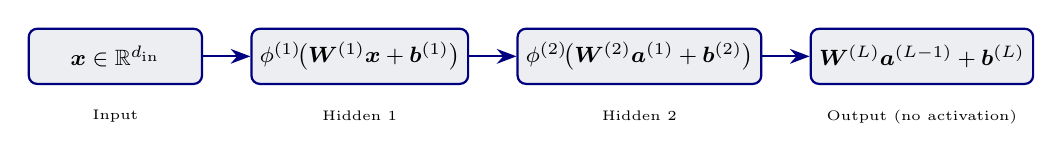
\begin{tikzpicture}[
    mlstep/.style={rectangle, draw=uzhblue, thick, fill=uzhgreylight,
        minimum width=2.2cm, minimum height=0.7cm, font=\footnotesize,
        rounded corners=3pt, inner sep=3pt},
    arr/.style={-{Stealth[length=2.5mm]}, thick, uzhblue}
]
    \node[mlstep] (in) {$\x \in \R^{d_{\text{in}}}$};
    \node[mlstep, right=0.6cm of in] (h1) {$\phi^{(1)}\!\bigl(\W^{(1)}\x + \bb^{(1)}\bigr)$};
    \node[mlstep, right=0.6cm of h1] (h2) {$\phi^{(2)}\!\bigl(\W^{(2)}\a^{(1)} + \bb^{(2)}\bigr)$};
    \node[mlstep, right=0.6cm of h2] (out) {$\W^{(L)}\a^{(L-1)} + \bb^{(L)}$};

    \draw[arr] (in) -- (h1);
    \draw[arr] (h1) -- (h2);
    \draw[arr] (h2) -- (out);

    \node[below=0.2cm, font=\tiny] at (in.south) {Input};
    \node[below=0.2cm, font=\tiny] at (h1.south) {Hidden 1};
    \node[below=0.2cm, font=\tiny] at (h2.south) {Hidden 2};
    \node[below=0.2cm, font=\tiny] at (out.south) {Output (no activation)};
\end{tikzpicture}
\end{center}

\vspace{0.3em}
Each hidden layer applies a \emphc{nonlinear activation} $\phi^{(\ell)}$:
\[
\a^{(\ell)} = \phi^{(\ell)}\!\bigl(\W^{(\ell)} \a^{(\ell-1)} + \bb^{(\ell)}\bigr), \qquad \ell = 1, \ldots, L-1
\]

\vspace{0.2em}
\begin{itemize}
    \item The output layer is typically \emphc{linear} (for regression) or uses \emphc{softplus} (to enforce positivity, e.g.\ consumption)
    \item The full network: $\mathcal{N}_\rho(\x) = \W^{(L)} \a^{(L-1)} + \bb^{(L)}$
\end{itemize}
\end{frame}

% --- Slide 16: Finding Parameters (Supervised) ---
\begin{frame}{Finding Parameters: Supervised Learning}
\textbf{Standard approach} (when labeled data $\{(\x_i, y_i)\}_{i=1}^N$ are available):

\vspace{0.5em}
\begin{enumerate}
    \item \textbf{Collect labeled data:}~~$\x_i \xrightarrow{\text{true mapping}} y_i$

    \vspace{0.3em}
    \item \textbf{Define a loss function:}
    \[
    \ell_\rho^{\text{sup}} = \frac{1}{N}\sum_{i=1}^{N} \bigl\|y_i - \mathcal{N}_\rho(\x_i)\bigr\|^2
    \qquad\text{(mean squared error)}
    \]

    \vspace{0.3em}
    \item \textbf{Update via SGD} ($\eta$ = learning rate; the symbol $\alpha$ is reserved for the Cobb--Douglas capital share later in the deck):
    \[
    \rho^{\text{new}} = \rho^{\text{old}} - \eta \cdot \frac{\partial \ell_\rho}{\partial \rho}\bigg|_{\rho = \rho^{\text{old}}}
    \]
\end{enumerate}

\vspace{0.3em}
{\small This is the recipe from Lecture~1. But in economics, \emphc{we rarely have labeled data}\ldots}
\end{frame}

% --- Slide 17: The Data Problem ---
\begin{frame}{The ``Data Problem'' in Economics}
\textbf{Deep learning excels} when massive labeled datasets are available.

\vspace{0.5em}
\textbf{But in computational economics:}
\begin{itemize}
    \item We solve \emphc{functional equations}, not classification/regression tasks
    \item There are \emphc{no labeled pairs} $(\x_i, y_i)$
    \item Traditional approach: \emphc{time iteration on a grid}, but grids do not scale
\end{itemize}

\vspace{0.5em}
\textbf{Key insight:}
\begin{itemize}
    \item We \emphc{know} the structural equations $G(\cdot) = 0$
    \item We can \emphc{check} how well a candidate policy satisfies them
    \item $\Rightarrow$ Use the \emphc{equilibrium error} as the loss function!
\end{itemize}
\end{frame}

% --- Slide 18: Issue with Time Iteration ---
\begin{frame}{Traditional Approach: Time Iteration on a Grid}
\begin{alertblock}{Algorithm: Grid-Based Collocation}
\begin{algorithmic}
\small
\STATE \textbf{Input:} Grid $\mathcal{G} = \{\x_1, \ldots, \x_M\} \subset \R^d$, initial guess $p^{(0)}$
\FOR{$k = 0, 1, 2, \ldots$ until convergence}
    \FOR{each grid point $\x_i \in \mathcal{G}$}
        \STATE Solve $G\bigl(\x_i,\, p^{(k)}(\x_i),\, p^{(k)}\bigr) = 0$ for $p^{(k+1)}(\x_i)$
    \ENDFOR
    \STATE Interpolate $p^{(k+1)}$ between grid points
\ENDFOR
\end{algorithmic}
\end{alertblock}

\vspace{0.3em}
\textbf{Problems:}
\begin{itemize}
    \item \emphc{Cartesian} grids need $M=n^d$ points, infeasible beyond $d\sim4\text{--}5$ at sensible resolution ($10^5$ at $d\!=\!5$, $10^{10}$ at $d\!=\!10$)
    \item \emphc{Sparse grids} (Smolyak, adaptive) extend the practical reach only to $d \sim 20\text{--}50$
    \item Heterogeneous-agent or many-country DSGE models routinely need $d \gg 50$, beyond any grid-based method
\end{itemize}
\end{frame}

% --- Slide 19: Economic Loss Function ---
\begin{frame}{The DEQN Loss Function}
\textbf{Key idea:} replace labeled data with \emphc{economic equilibrium conditions}.

\vspace{0.5em}
Let $G(\x, f(\x)) = 0$ be the system of equilibrium equations. Define:
\[
\boxed{
\ell_\rho = \frac{1}{N} \sum_{i=1}^{N} \bigl\| G\bigl(\x_i,\, \mathcal{N}_\rho(\x_i)\bigr) \bigr\|^2
}
\]

\vspace{0.3em}
\begin{itemize}
    \item $\mathcal{N}_\rho(\x_i)$ is the neural net's \emphc{predicted policy} at state $\x_i$
    \item $G(\cdot)$ measures the \emphc{equilibrium error} (e.g.\ Euler equation residual)
    \item Small $\ell_\rho$ means the policy nearly satisfies the equations on the sampled states
\end{itemize}

\vspace{0.5em}
$\Rightarrow$ \emphc{No labels needed}, so this is \textbf{unsupervised} (or ``self-supervised'') learning.
\\[2pt]
{\scriptsize In stochastic models, expectations inside $G$ are approximated, e.g.\ by path averaging or quadrature.}
\end{frame}

% --- Slide 20: Inside one DEQN step ---
\begin{frame}{Inside One DEQN Training Step}
\begin{center}
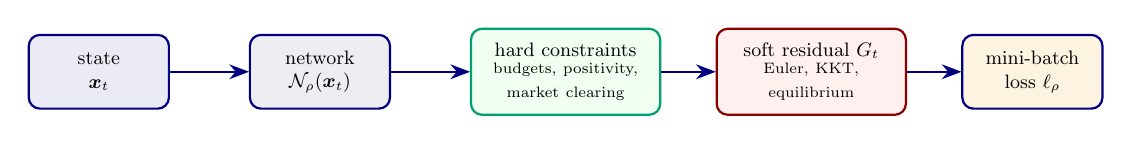
\begin{tikzpicture}[scale=0.78, transform shape,
    box/.style={rectangle, draw=uzhblue, thick, rounded corners=4pt,
                text width=2.0cm, minimum height=1.2cm, align=center, font=\small, inner sep=4pt},
    hard/.style={rectangle, draw=softgreen, thick, rounded corners=4pt,
                fill=green!6, text width=2.8cm, minimum height=1.4cm, align=center, font=\small, inner sep=4pt},
    soft/.style={rectangle, draw=darkred, thick, rounded corners=4pt,
                fill=red!6, text width=2.8cm, minimum height=1.4cm, align=center, font=\small, inner sep=4pt},
    arr/.style={-{Stealth[length=2.5mm]}, thick, uzhblue}
]
    \node[box, fill=uzhblue!8]    (x)    at ( 0.0, 0) {state\\$\x_t$};
    \node[box, fill=uzhgreylight] (nn)   at ( 3.6, 0) {network\\$\mathcal{N}_\rho(\x_t)$};
    \node[hard]                   (hc)   at ( 7.6, 0) {hard constraints\\\scriptsize budgets, positivity,\\\scriptsize market clearing};
    \node[soft]                   (res)  at (11.6, 0) {soft residual $G_t$\\\scriptsize Euler, KKT,\\\scriptsize equilibrium};
    \node[box, fill=softorange!12](loss) at (15.2, 0) {mini-batch\\loss $\ell_\rho$};

    \draw[arr] (x)   -- (nn);
    \draw[arr] (nn)  -- (hc);
    \draw[arr] (hc)  -- (res);
    \draw[arr] (res) -- (loss);
\end{tikzpicture}
\end{center}

\vspace{0.4em}
\begin{itemize}
    \item Encode what can be enforced \emphc{exactly} in the architecture.
    \item Minimize only the genuinely non-closed-form equilibrium conditions.
    \item Draw states from the model's own simulation, so training focuses on the ergodic set.
\end{itemize}
\end{frame}

% --- Slide 21: Training DEQN Algorithm ---
\begin{frame}{Training Algorithm for DEQNs}
\begin{block}{Algorithm 1: Deep Equilibrium Net Training}
\begin{algorithmic}
\footnotesize
\STATE \textbf{Input:} Initial state $\x_0$, network $\mathcal{N}_\rho$, learning rate $\eta$, episodes $E$, simulation horizon $T_{\mathrm{sim}}$, training steps $T_{\mathrm{train}}$
\FOR{episode $e = 1, \ldots, E$}
    \STATE \textbf{Simulate path:} $\x_0 \to \x_1 \to \cdots \to \x_{T_{\mathrm{sim}}}$ using $\mathcal{N}_\rho$ and transition law
    \FOR{gradient step $t = 1, \ldots, T_{\mathrm{train}}$}
        \STATE Draw mini-batch $\mathcal{B} \subset \{\x_0, \ldots, \x_{T_{\mathrm{sim}}}\}$
        \STATE Compute loss:~$\ell_\rho = \frac{1}{|\mathcal{B}|}\sum_{\x_i \in \mathcal{B}} \|G(\x_i, \mathcal{N}_\rho(\x_i))\|^2$
        \STATE Update:~$\rho \leftarrow \rho - \eta \cdot \nabla_\rho \ell_\rho$
    \ENDFOR
\ENDFOR
\STATE \textbf{Output:} Trained network $\mathcal{N}_{\rho^\star}$ approximating the policy function
\end{algorithmic}
\end{block}

\vspace{0.2em}
{\small \textbf{Note:} Training points come from the \emphc{model's own simulation}, so the network learns on the ergodic distribution, focusing on economically relevant regions.}
\end{frame}

% --- Slide 21: Supervised vs Unsupervised ---
\begin{frame}{Supervised vs.\ Unsupervised (DEQN) Learning}
\begin{columns}[T]
\column{0.47\textwidth}
\begin{center}
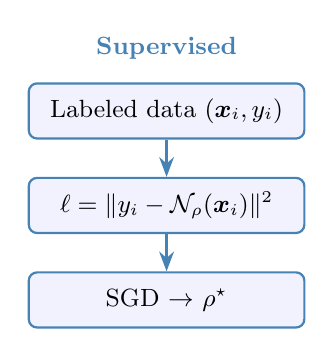
\begin{tikzpicture}[
    mlstep/.style={rectangle, draw=softblue, thick, fill=blue!5,
        minimum width=3.5cm, minimum height=0.7cm, font=\small,
        rounded corners=3pt},
    arr/.style={-{Stealth[length=2.5mm]}, thick, softblue}
]
    \node[font=\small\bfseries, softblue] at (0,3.2) {Supervised};
    \node[mlstep] (d) at (0,2.4) {Labeled data $(\x_i, y_i)$};
    \node[mlstep] (l) at (0,1.2) {$\ell = \|y_i - \mathcal{N}_\rho(\x_i)\|^2$};
    \node[mlstep] (s) at (0,0) {SGD $\to$ $\rho^\star$};
    \draw[arr] (d) -- (l);
    \draw[arr] (l) -- (s);
\end{tikzpicture}
\end{center}

\column{0.47\textwidth}
\begin{center}
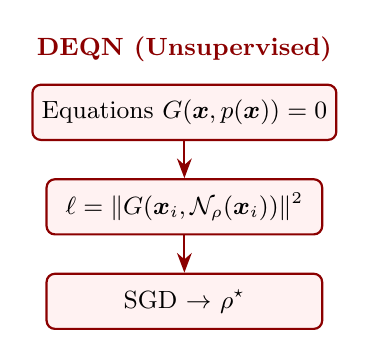
\begin{tikzpicture}[
    mlstep/.style={rectangle, draw=darkred, thick, fill=red!5,
        minimum width=3.5cm, minimum height=0.7cm, font=\small,
        rounded corners=3pt},
    arr/.style={-{Stealth[length=2.5mm]}, thick, darkred}
]
    \node[font=\small\bfseries, darkred] at (0,3.2) {DEQN (Unsupervised)};
    \node[mlstep] (d) at (0,2.4) {Equations $G(\x, p(\x))=0$};
    \node[mlstep] (l) at (0,1.2) {$\ell = \|G(\x_i, \mathcal{N}_\rho(\x_i))\|^2$};
    \node[mlstep] (s) at (0,0) {SGD $\to$ $\rho^\star$};
    \draw[arr] (d) -- (l);
    \draw[arr] (l) -- (s);
\end{tikzpicture}
\end{center}
\end{columns}

\vspace{0.5em}
\begin{center}
{\small \emphc{Key difference:} DEQNs replace labeled data with structural economic equations.}
\end{center}
\end{frame}

% --- Slide 22: DEQN Key Recap ---
\begin{frame}{DEQN: Key Recap}
\begin{columns}[T]
\column{0.32\textwidth}
\begin{block}{Replace Labels}
\centering
\small
Instead of labeled data $(\x_i, y_i)$, use the economic equilibrium equations $G(\cdot) = 0$ as the loss.
\end{block}

\column{0.32\textwidth}
\begin{block}{Replace Grids}
\centering
\small
Instead of $n^d$ grid points, use a neural network $\mathcal{N}_\rho$ that maps states to policies \emphc{globally}.
\end{block}

\column{0.32\textwidth}
\begin{block}{Replace TI}
\centering
\small
Instead of time iteration with interpolation, use SGD on simulated paths from the model.
\end{block}
\end{columns}

\vspace{0.8em}
\begin{center}
\textbf{Result:} A grid-free, simulation-based method that can handle
much higher-dimensional models than standard grids and maps naturally to GPUs.
\end{center}
\end{frame}

% ============================================================================
% PART III: BROCK--MIRMAN BENCHMARK
% ============================================================================

% --- Slide 23: Section Divider ---
\begin{frame}{}
\vfill
\begin{center}
{\Huge \textcolor{uzhblue}{\textbf{Part III}}}\\[12pt]
{\LARGE Brock--Mirman Benchmark}
\end{center}
\vfill
\end{frame}

% --- Slide 24: Brock-Mirman Setup ---
\begin{frame}{Brock--Mirman (1972): Setup}
\footnotesize
\textbf{Social planner's problem.} Choose a consumption sequence to maximize expected lifetime log utility:
\[
\max_{\{C_t\}_{t=0}^{\infty}} \; \E{\sum_{t=0}^{\infty} \beta^t \ln C_t}
\]

\vspace{0.2em}
\textbf{Resource constraint} (full depreciation, $\delta = 1$):
\[
C_t + K_{t+1} \;=\; z_t K_t^{\alpha}, \qquad K_0 > 0 \text{ given.}
\]

\vspace{0.2em}
\textbf{Stochastic productivity.} TFP $z_t$ follows an AR(1) in logs:
\[
\ln z_{t+1} \;=\; \varrho \ln z_t + \sigma_z\, \epsilon_{t+1}, \qquad \epsilon_{t+1} \sim \mathcal{N}(0,1).
\]

\vspace{0.2em}
\textbf{State \& control.} State $\bm{x}_t = (K_t, z_t)$; control $C_t$. Capital then follows from the budget as $K_{t+1} = z_t K_t^\alpha - C_t$.

\vspace{0.4em}
{\footnotesize\emphc{Next two slides:} derive the Euler equation from first principles, then obtain the closed-form policy -- the benchmark we will later compare the DEQN solution to.}
\end{frame}

% --- Slide 25: Deriving the Euler equation (Lagrangian) ---
\begin{frame}{Deriving the Euler Equation (Lagrangian)}
\footnotesize
\textbf{Step 1. Lagrangian.} Attach a multiplier $\lambda_t \ge 0$ to each period's budget constraint:
\[
\mathcal{L} \;=\; \E{\sum_{t=0}^{\infty} \beta^t \Big[\, \ln C_t \;-\; \lambda_t\,\big( C_t + K_{t+1} - z_t K_t^{\alpha} \big) \Big]}.
\]

\vspace{0.2em}
\textbf{Step 2. Take partial derivatives} with respect to the choices at date $t$:
\begin{columns}[T]
\column{0.48\textwidth}
\emphc{Consumption FOC} $\;\partial\mathcal{L}/\partial C_t = 0$:
\[
\beta^t\!\left( \frac{1}{C_t} - \lambda_t \right) = 0
\;\;\Longrightarrow\;\; \lambda_t = \frac{1}{C_t}.
\]

\column{0.52\textwidth}
\emphc{Capital FOC} $\;\partial\mathcal{L}/\partial K_{t+1} = 0$:
\[
-\beta^t \lambda_t \;+\; \beta^{t+1}\,\E{\lambda_{t+1}\,\alpha z_{t+1} K_{t+1}^{\alpha-1}} = 0.
\]
\end{columns}

\vspace{0.3em}
\textbf{Step 3. Eliminate $\lambda$.} Substitute $\lambda_t = 1/C_t$, $\lambda_{t+1} = 1/C_{t+1}$ and divide by $\beta^t$:
\[
\boxed{\;\; \frac{1}{C_t} \;=\; \beta\, \E{\frac{\alpha\, z_{t+1}\, K_{t+1}^{\alpha-1}}{C_{t+1}}} \;\;} \quad \text{(stochastic Euler equation)}
\]

\vspace{0.2em}
{\scriptsize\emphc{Reading:} marginal utility of today's consumption $\; = \;$ discounted expected marginal utility of tomorrow's consumption $\,\times\,$ gross marginal product of capital at $t{+}1$. The transversality condition $\lim_{t\to\infty}\E{\beta^t \lambda_t K_{t+1}} = 0$ rules out bubbles.}
\end{frame}

% --- Slide 26: Closed-form policy (guess-and-verify) ---
\begin{frame}{Closed-Form Policy via Guess-and-Verify}
\footnotesize
\textbf{Guess.} Consumption is a constant fraction $1-\phi$ of output:
\[
C_t \;=\; (1-\phi)\, z_t K_t^{\alpha}, \qquad \phi \in (0,1)\ \text{to be determined.}
\]
The budget then implies $K_{t+1} = \phi\, z_t K_t^{\alpha}$.

\vspace{0.2em}
\textbf{Substitute into the Euler equation.} With $C_{t+1} = (1-\phi)\, z_{t+1} K_{t+1}^{\alpha}$,
\[
\frac{\alpha\, z_{t+1}\, K_{t+1}^{\alpha-1}}{C_{t+1}}
\;=\; \frac{\alpha\, z_{t+1}\, K_{t+1}^{\alpha-1}}{(1-\phi)\, z_{t+1}\, K_{t+1}^{\alpha}}
\;=\; \frac{\alpha}{(1-\phi)\, K_{t+1}}.
\]
\emphc{Note:} $z_{t+1}$ cancels, so the conditional expectation collapses (log $+$ Cobb--Douglas $+$ full depreciation).

\vspace{0.2em}
\textbf{Solve for $\phi$.} Plug $K_{t+1} = \phi z_t K_t^\alpha$ on both sides of the Euler:
\[
\underbrace{\frac{1}{(1-\phi)\, z_t K_t^{\alpha}}}_{\text{LHS}}
\;=\; \beta\, \cdot\, \underbrace{\frac{\alpha}{(1-\phi)\, \phi\, z_t K_t^{\alpha}}}_{\text{RHS}}
\;\;\Longrightarrow\;\; 1 = \frac{\beta\alpha}{\phi}
\;\;\Longrightarrow\;\; \phi = \beta\alpha.
\]

\vspace{0.2em}
\textbf{Closed-form policy.}
\[
\boxed{\;\; C_t \;=\; (1-\beta\alpha)\, z_t K_t^{\alpha},
\qquad K_{t+1} \;=\; \beta\alpha\, z_t K_t^{\alpha} \;\;}
\]

{\scriptsize This benchmark provides an analytic target against which we will measure the DEQN's trained policy.}
\end{frame}

\end{document}
